\subsection{Description du déroulement projet}

Dans cette section, nous allons retracer le déroulement du projet au travers de l'analyse des burndown charts de chacun des sprints.

\subsubsection{Sprint 1}

\begin{figure}[h]
\begin{center}
	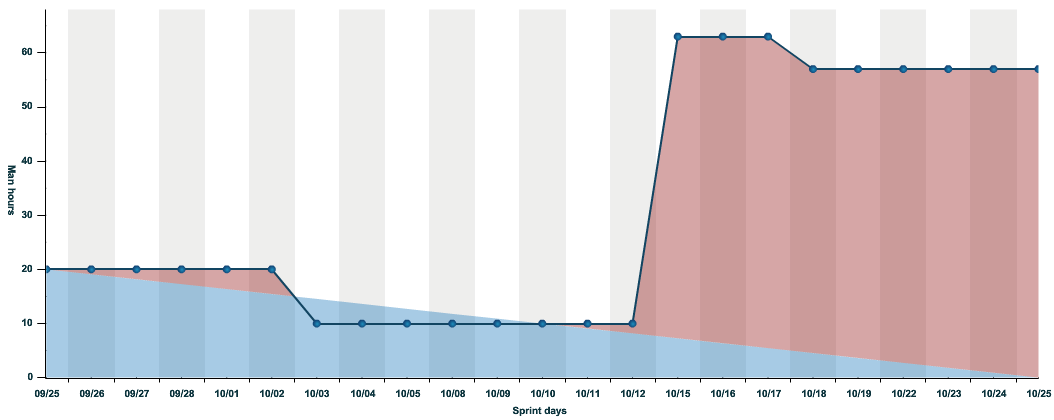
\includegraphics[width=11cm]{burndown-S1.png}
\end{center}
	\caption{Burdown chart du sprint 1}
\end{figure}

L'activité principale de ce premier sprint a été de créer une couche modèle pour notre application. Ceci impliquait de trouver une bibliothèque permettant de lire le format dicom et qui soit compatible avec android. Cette tache a demandé beaucoup d'investissement et de recherche et n'a pu être achevée qu'au sprint suivant. C'est pourquoi on remarque trois plateaux de stagnation. L'augmentation spectaculaire du nombre d'homme-heure restant vers la fin du sprint est du à une mauvaise utilisation de l'outil. En effet, ce sprint nous a introduit à la méthode \emph{scrum} et aux outils associés. De ce fait, notre manque d'assurance et de maitrise explique les imperfections de ce sprint. Néanmoins, on constate tout de même que des avancées significatives ont pu être réalisées durant ce sprint, la partie modèle étant en majorité achevée lors du passage au deuxième sprint.